\documentclass[final]{beamer}

% ====================
% PACKAGES
% ====================
\usepackage[orientation=portrait,size=a3,scale=1.25,debug]{beamerposter}
\usepackage[utf8]{inputenc}
\usepackage{amsmath, amsthm, amssymb, amsfonts}
\usepackage{graphicx}
\usepackage{booktabs}
\usepackage{tcolorbox}
\usepackage{ragged2e}
\usepackage{tikz}
\usetikzlibrary{shapes,arrows,positioning,calc,fit,backgrounds}

% ====================
% THEME & COLORS
% ====================
\mode<presentation> {
  \usetheme{Madrid}
  \usecolortheme{beaver}
}

\definecolor{kuRed}{RGB}{164, 16, 52}
\definecolor{kuGrey}{RGB}{70, 70, 70}
\definecolor{voltGreen}{RGB}{46, 204, 113}
\definecolor{sgdRed}{RGB}{214, 39, 40}
\definecolor{streamBlue}{RGB}{31, 119, 180}

\setbeamercolor{palette primary}{bg=kuRed,fg=white}
\setbeamercolor{palette secondary}{bg=kuRed,fg=white}
\setbeamercolor{palette tertiary}{bg=kuRed,fg=white}
\setbeamercolor{palette quaternary}{bg=kuRed,fg=white}
\setbeamercolor{structure}{fg=kuRed}
\setbeamercolor{titlelike}{parent=palette primary,fg=white}
\setbeamercolor{frametitle}{bg=kuGrey,fg=white}
\setbeamertemplate{footline}{}
\setbeamertemplate{navigation symbols}{}

\setbeamerfont{block title}{size=\large, series=\bfseries}
\setbeamerfont{block body}{size=\normalsize}

% ====================
% TITLE
% ====================
\title{}
\author{}
\institute{}
\date{}

% ====================
% DOCUMENT
% ====================
\begin{document}
\begin{frame}[t]

% ====================
% HEADER: Logo Left, Title Right
% Logo is 1280x335 (ratio 3.82:1). At 0.18\linewidth width, height ~ 1.2cm
% ====================
\begin{columns}[T]
    \begin{column}{0.18\linewidth}
        
\includegraphics[width=\linewidth]{ku_logo.png}
    \end{column}
    \begin{column}{0.80\linewidth}
        \begin{beamercolorbox}[wd=\linewidth,ht=1.2cm,dp=0.2cm,center]{palette primary}
            {\Large \textbf{Testing the Volterra Model for SGD on Real Data}}\\[0.08cm]
            {\small Kaan Alta\c{s} \& Yi\u{g}it Karasu \hfill ELEC/COMP 450 \hfill Instructor: Asst. Prof. Zafer Do\u{g}an}
        \end{beamercolorbox}
    \end{column}
\end{columns}

\vspace{0.2cm}

% ====================
% CONTENT
% ====================
\begin{columns}[t]

% ==================== LEFT COLUMN ====================
\begin{column}{0.48\linewidth}

% --- 1. PROBLEM CONTEXT ---
\begin{block}{1. Problem Context \& Motivation}
\justifying
\textbf{SGD} is the workhorse of modern machine learning, yet its dynamics remain poorly understood. The paper \textit{``SGD in the Large''} (Paquette et al., NeurIPS 2021) provides an \textbf{exact deterministic prediction} of SGD's training loss using \textbf{Volterra integral equations}.

\vspace{0.2cm}
\textbf{Key Question:} The theory assumes \textit{isotropic} (Gaussian) data. \textbf{Does it work on real data like MNIST?}

\vspace{0.2cm}
\textbf{Our Contribution:}
\begin{itemize}
    \item Replicate paper's Figure 4 (synthetic data validation)
    \item Test Volterra on \textbf{MNIST random features} with real labels
    \item Analyze \textbf{non-linear targets} and \textbf{whitening} effects
    \item Study \textbf{step-size criticality} on real eigenvalue spectra
\end{itemize}
\end{block}

% --- 2. THEORETICAL FRAMEWORK ---
\begin{block}{2. Theoretical Framework}
\justifying
\textbf{Least Squares Problem:}
\vspace{-0.2cm}
$$\min_{\mathbf{x} \in \mathbb{R}^d} f(\mathbf{x}) = \frac{1}{2n} \|A\mathbf{x} - \mathbf{b}\|^2$$

\textbf{SGD Update Rule} (with rescaled step size $\gamma$):
\vspace{-0.2cm}
$$\mathbf{x}_{k+1} = \mathbf{x}_k - \frac{\gamma}{n} \nabla f_{i_k}(\mathbf{x}_k), \quad i_k \sim \text{Uniform}[n]$$

\textbf{Main Result --- Volterra Integral Equation:}\\
As $n, d \to \infty$ with $r = d/n$ fixed, the expected loss $\mathbb{E}[f(\mathbf{x}_t)]$ converges to $\psi_0(t)$:
\vspace{-0.1cm}
$$\boxed{\psi_0(t) = z(t) + r\gamma^2 \int_0^t h_2(t-s) \psi_0(s) \, ds}$$

where $h_2(t)$ is determined by the \textbf{eigenvalue distribution} of $H = \frac{1}{n}A^\top A$.

\vspace{0.2cm}
\textbf{Critical Step Size} (stability threshold):
\vspace{-0.2cm}
$$\gamma_{\max} = \frac{2}{r} \cdot \frac{1}{\bar{\lambda}}, \quad \bar{\lambda} = \frac{1}{d}\sum_{i=1}^d \lambda_i$$
\end{block}

% --- 3. EXPERIMENTAL SETTINGS ---
\begin{block}{3. Experimental Settings}
\justifying

% TikZ Diagram for Settings
\begin{center}
\begin{tikzpicture}[
    box/.style={rectangle, draw=kuGrey, thick, minimum width=2.8cm, minimum height=1.2cm, align=center, font=\small},
    arrow/.style={->, thick, >=stealth},
    label/.style={font=\footnotesize\bfseries}
]
% Row 1: Data Generation
\node[box, fill=blue!10] (mnist) at (0,0) {MNIST\\$X \in \mathbb{R}^{n \times 784}$};
\node[box, fill=green!10] (rf) at (4,0) {Random Features\\$A = \sigma(XW)$};
\node[box, fill=orange!10] (target) at (8,0) {Target $\mathbf{b}$};

\draw[arrow] (mnist) -- (rf) node[midway, above, font=\scriptsize] {$W \in \mathbb{R}^{784 \times d}$};
\draw[arrow] (rf) -- (target);

% Settings below
\node[below=0.3cm of mnist, font=\scriptsize, align=center] {$n = 3000$ samples\\Real digit images};
\node[below=0.3cm of rf, font=\scriptsize, align=center] {$d = rn$ features\\$\sigma$ = Shifted ReLU};
\node[below=0.3cm of target, font=\scriptsize, align=center] {$r \in \{0.5, 1.0, 1.5\}$\\Aspect ratios};
\end{tikzpicture}
\end{center}

\vspace{0.2cm}
\textbf{Three Target Settings:}
\vspace{-0.1cm}
\begin{center}
\renewcommand{\arraystretch}{1.3}
\begin{tabular}{lll}
\toprule
\textbf{Setting} & \textbf{Target Formula} & \textbf{Purpose} \\
\midrule
\textcolor{sgdRed}{\textbf{Base (Linear)}} & $\mathbf{b} = A\mathbf{x}^*$ & Realizable, matches theory \\
\textcolor{streamBlue}{\textbf{Nonlinear}} & $\mathbf{b} = \text{ReLU}(A\mathbf{x}^*)$ & Non-realizable stress test \\
\textcolor{voltGreen}{\textbf{Whitened}} & $\tilde{A} = A\Sigma^{-1/2}$ & Closer to isotropic assumption \\
\bottomrule
\end{tabular}
\end{center}

\vspace{0.1cm}
\textbf{Tools:} PyTorch \quad \textbf{Data:} Gaussian (replication), MNIST (new results)
\end{block}

% --- 4. REPLICATION RESULTS ---
\begin{block}{4. Replication Results (Paper Figure 4)}
\justifying
We compare 5 models: \textbf{Empirical SGD}, \textbf{Volterra}, \textbf{Streaming}, \textbf{SME}, \textbf{SDE}.

\vspace{0.2cm}
% fig1: 2361x1761 (1.34:1), paper: 1376x1268 (1.09:1) - use height to align
\begin{columns}[T]
\begin{column}{0.52\linewidth}
\centering

\includegraphics[height=4.5cm]{fig1_replication.png}\\
\scriptsize Our Replication
\end{column}
\begin{column}{0.46\linewidth}
\centering
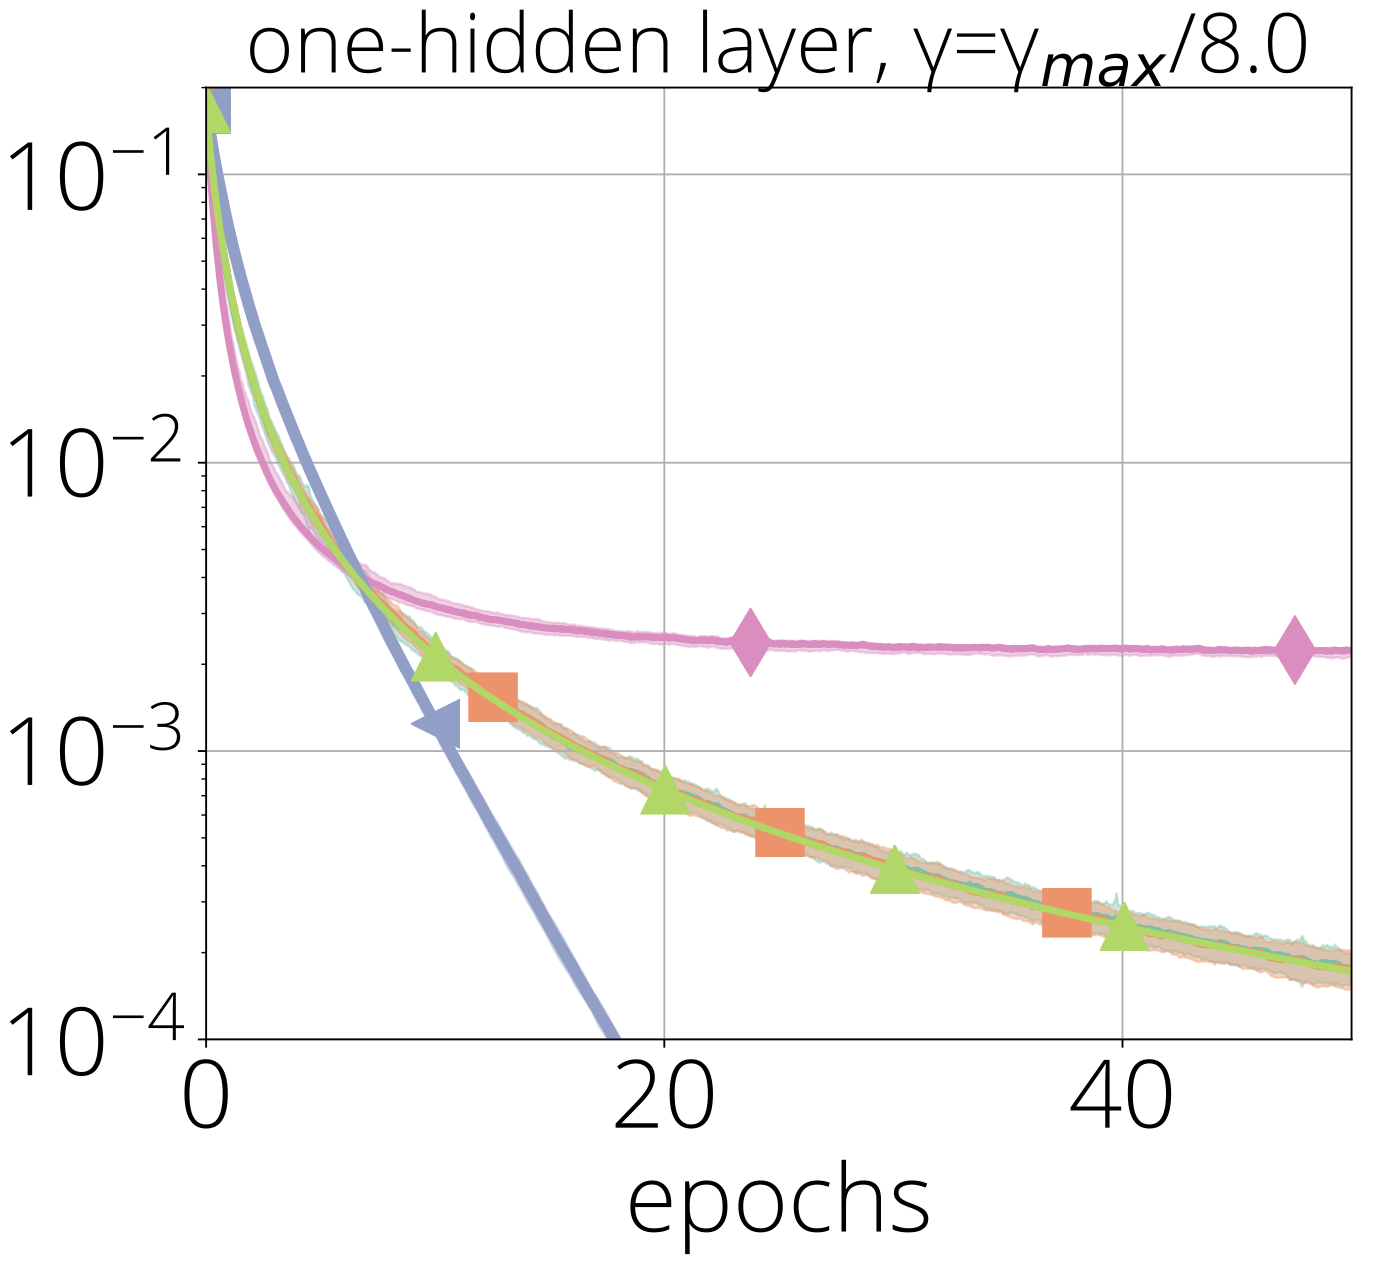
\includegraphics[height=4.5cm]{paper_result.png}\\
\scriptsize Original Paper (Fig. 4)
\end{column}
\end{columns}

\vspace{0.1cm}
\textbf{Observation:} Volterra (green) accurately predicts SGD. SDE underestimates due to isotropic noise. Streaming decreases further (infinite data).
\end{block}

% --- KEY FINDINGS ---
\begin{block}{Key Findings}
\justifying
\begin{itemize}
    \item \textbf{Volterra works on real data:} $R > 0.97$ even for non-linear targets
    \item \textbf{Spectral ratio matters:} MNIST has $\lambda_{\max}/\bar{\lambda} \sim 170$ vs. theory assumes $\approx 1$
    \item \textbf{Whitening helps:} Reduces spectral ratio by $\sim$4x, achieving $R \approx 0.999$
    \item \textbf{Critical step size gap:} Theory overestimates safe $\gamma$ by $\sim$100x
\end{itemize}
\end{block}

% --- REFERENCES ---
\begin{block}{References}
\footnotesize
\begin{thebibliography}{9}
\bibitem{paquette2021} Paquette et al. (2021). \textit{SGD in the Large: Average-case Analysis, Asymptotics, and Stepsize Criticality}. NeurIPS.
\end{thebibliography}
\end{block}

\end{column}

% ==================== RIGHT COLUMN ====================
\begin{column}{0.48\linewidth}

% --- 6. NEW RESULTS ---
\begin{block}{5. MNIST Random Features}
\justifying

\textbf{(a) Base Setting:} Linear target $\mathbf{b} = A\mathbf{x}^*$ --- Realizable
\vspace{0.1cm}
\begin{center}
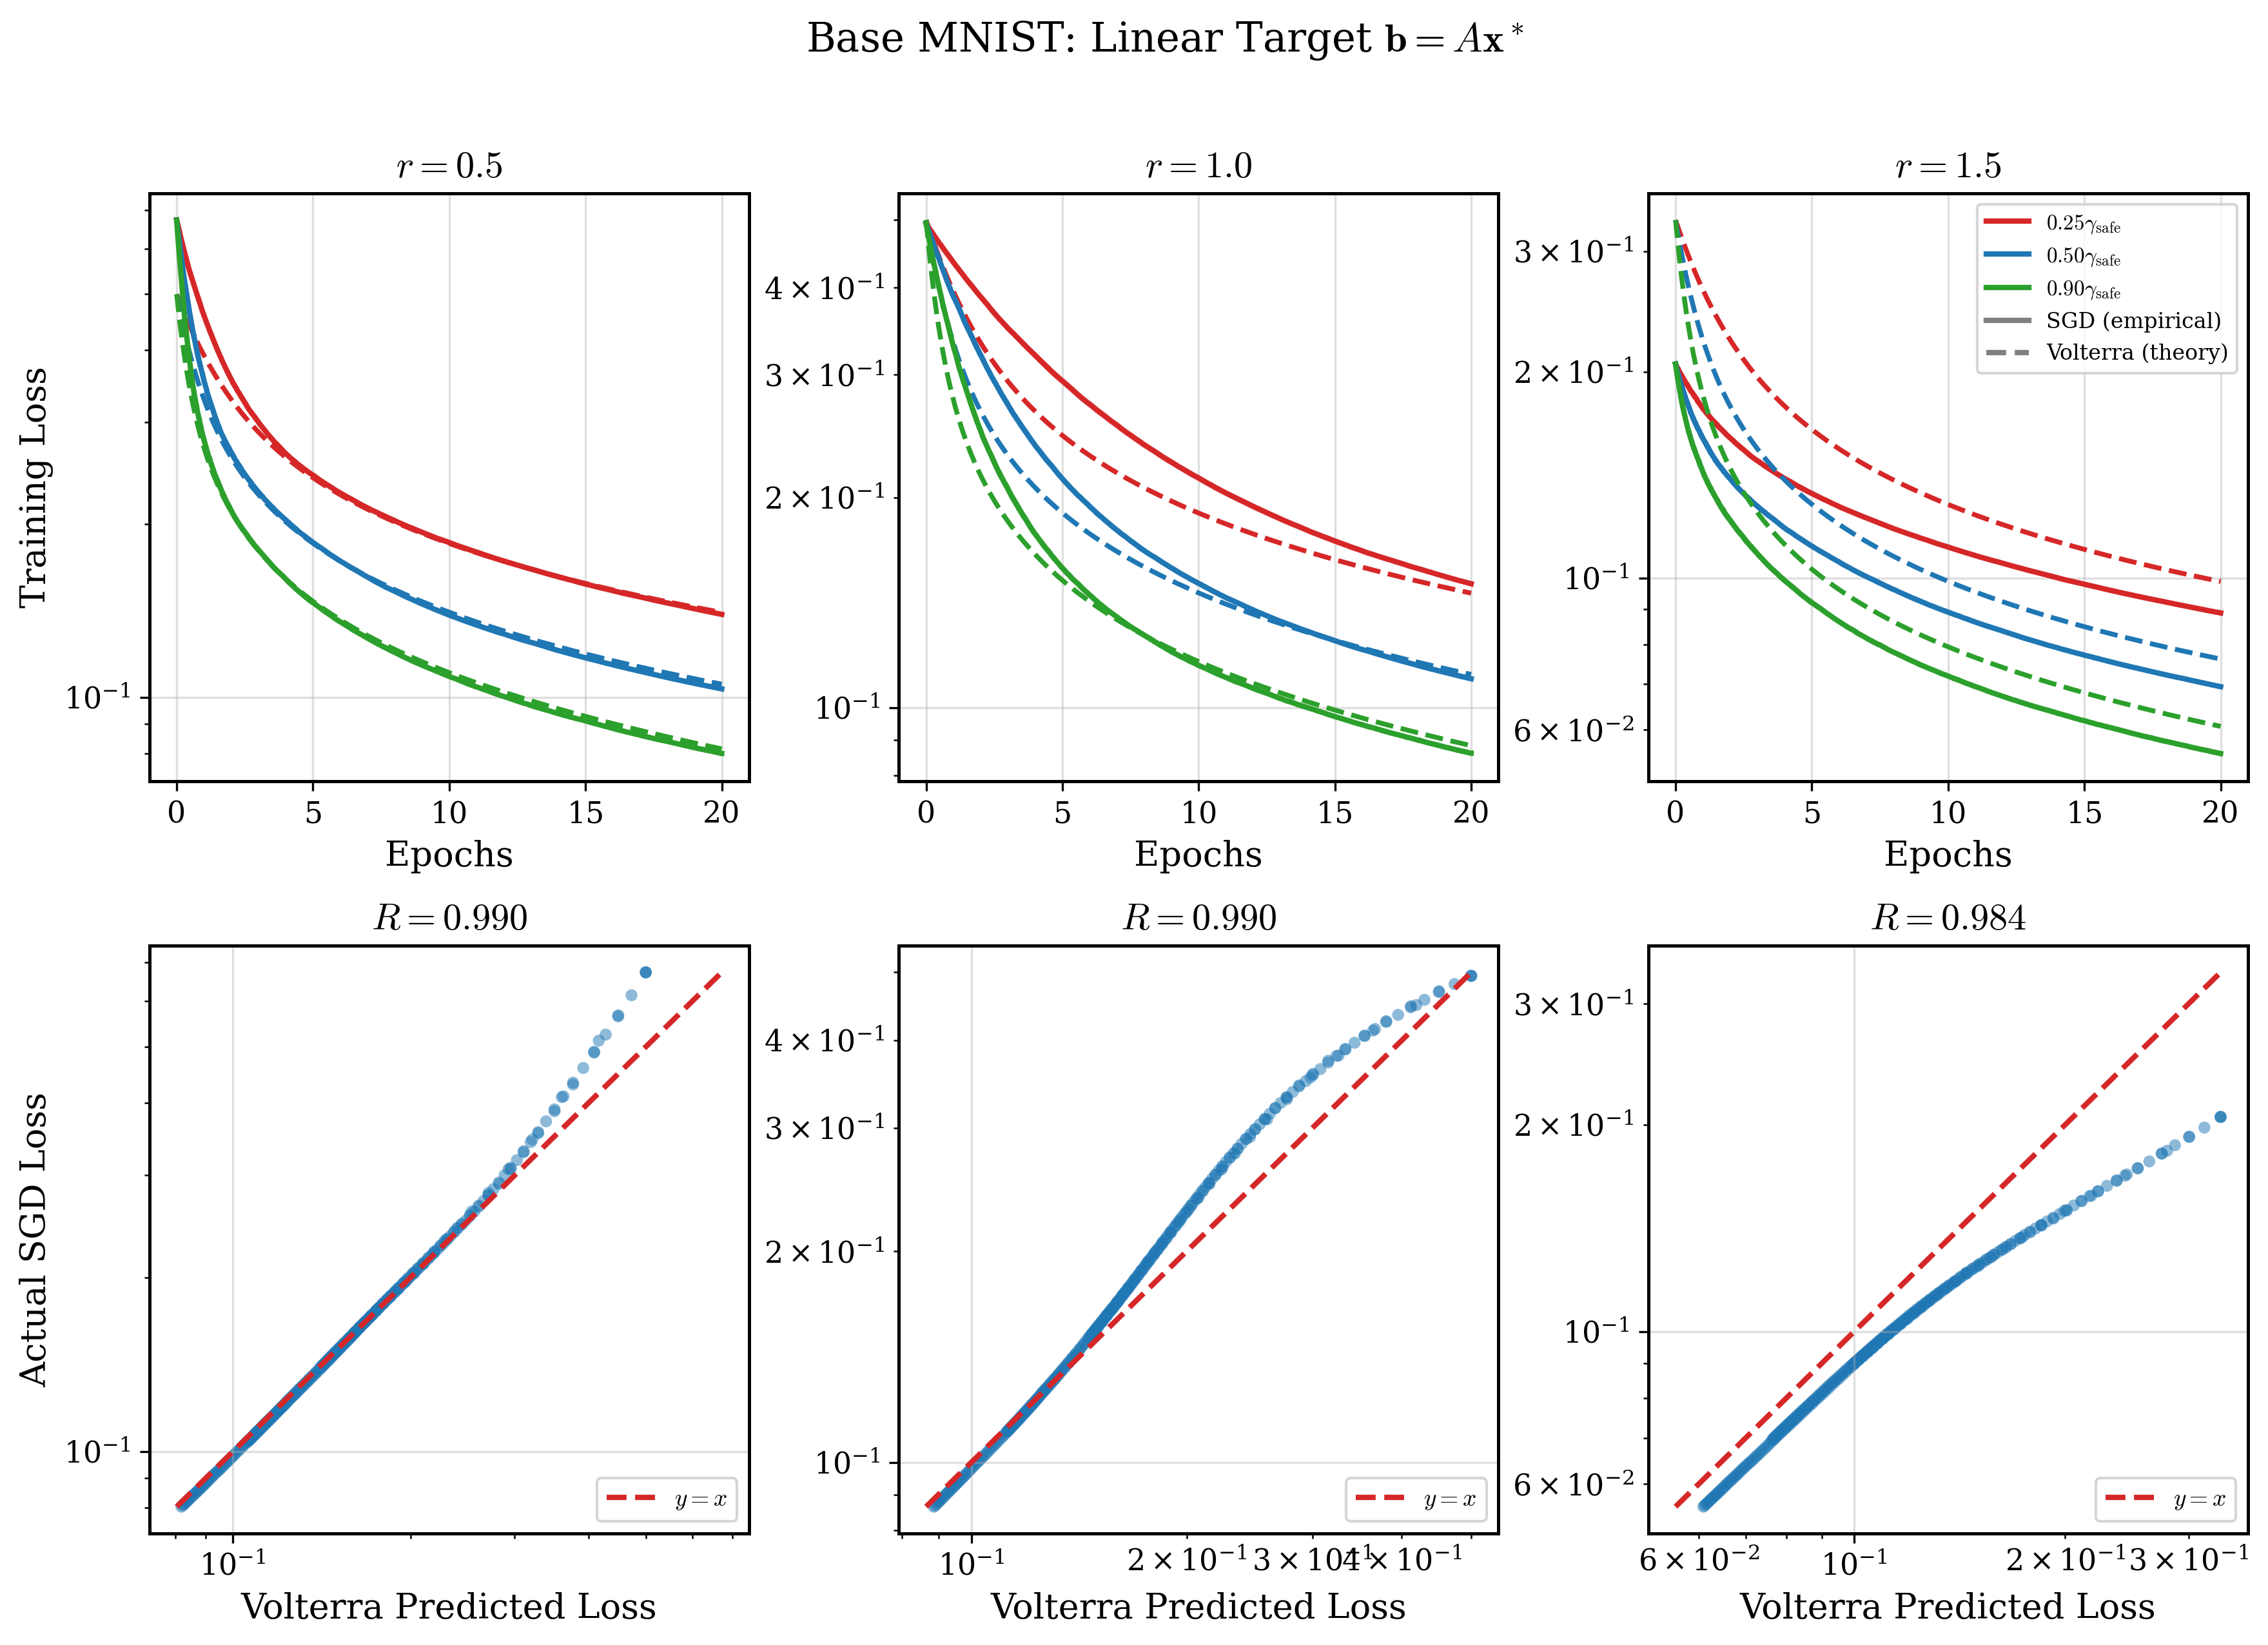
\includegraphics[width=0.95\linewidth]{fig2_base_mnist.png}
\end{center}
\vspace{-0.2cm}
\small \textit{Top: Loss curves (solid=SGD, dashed=Volterra). Bottom: Correlation $R > 0.98$.}

\vspace{0.3cm}
\textbf{(b) Nonlinear Setting:} $\mathbf{b} = \text{ReLU}(A\mathbf{x}^*)$ --- Non-realizable
\vspace{0.1cm}
\begin{center}
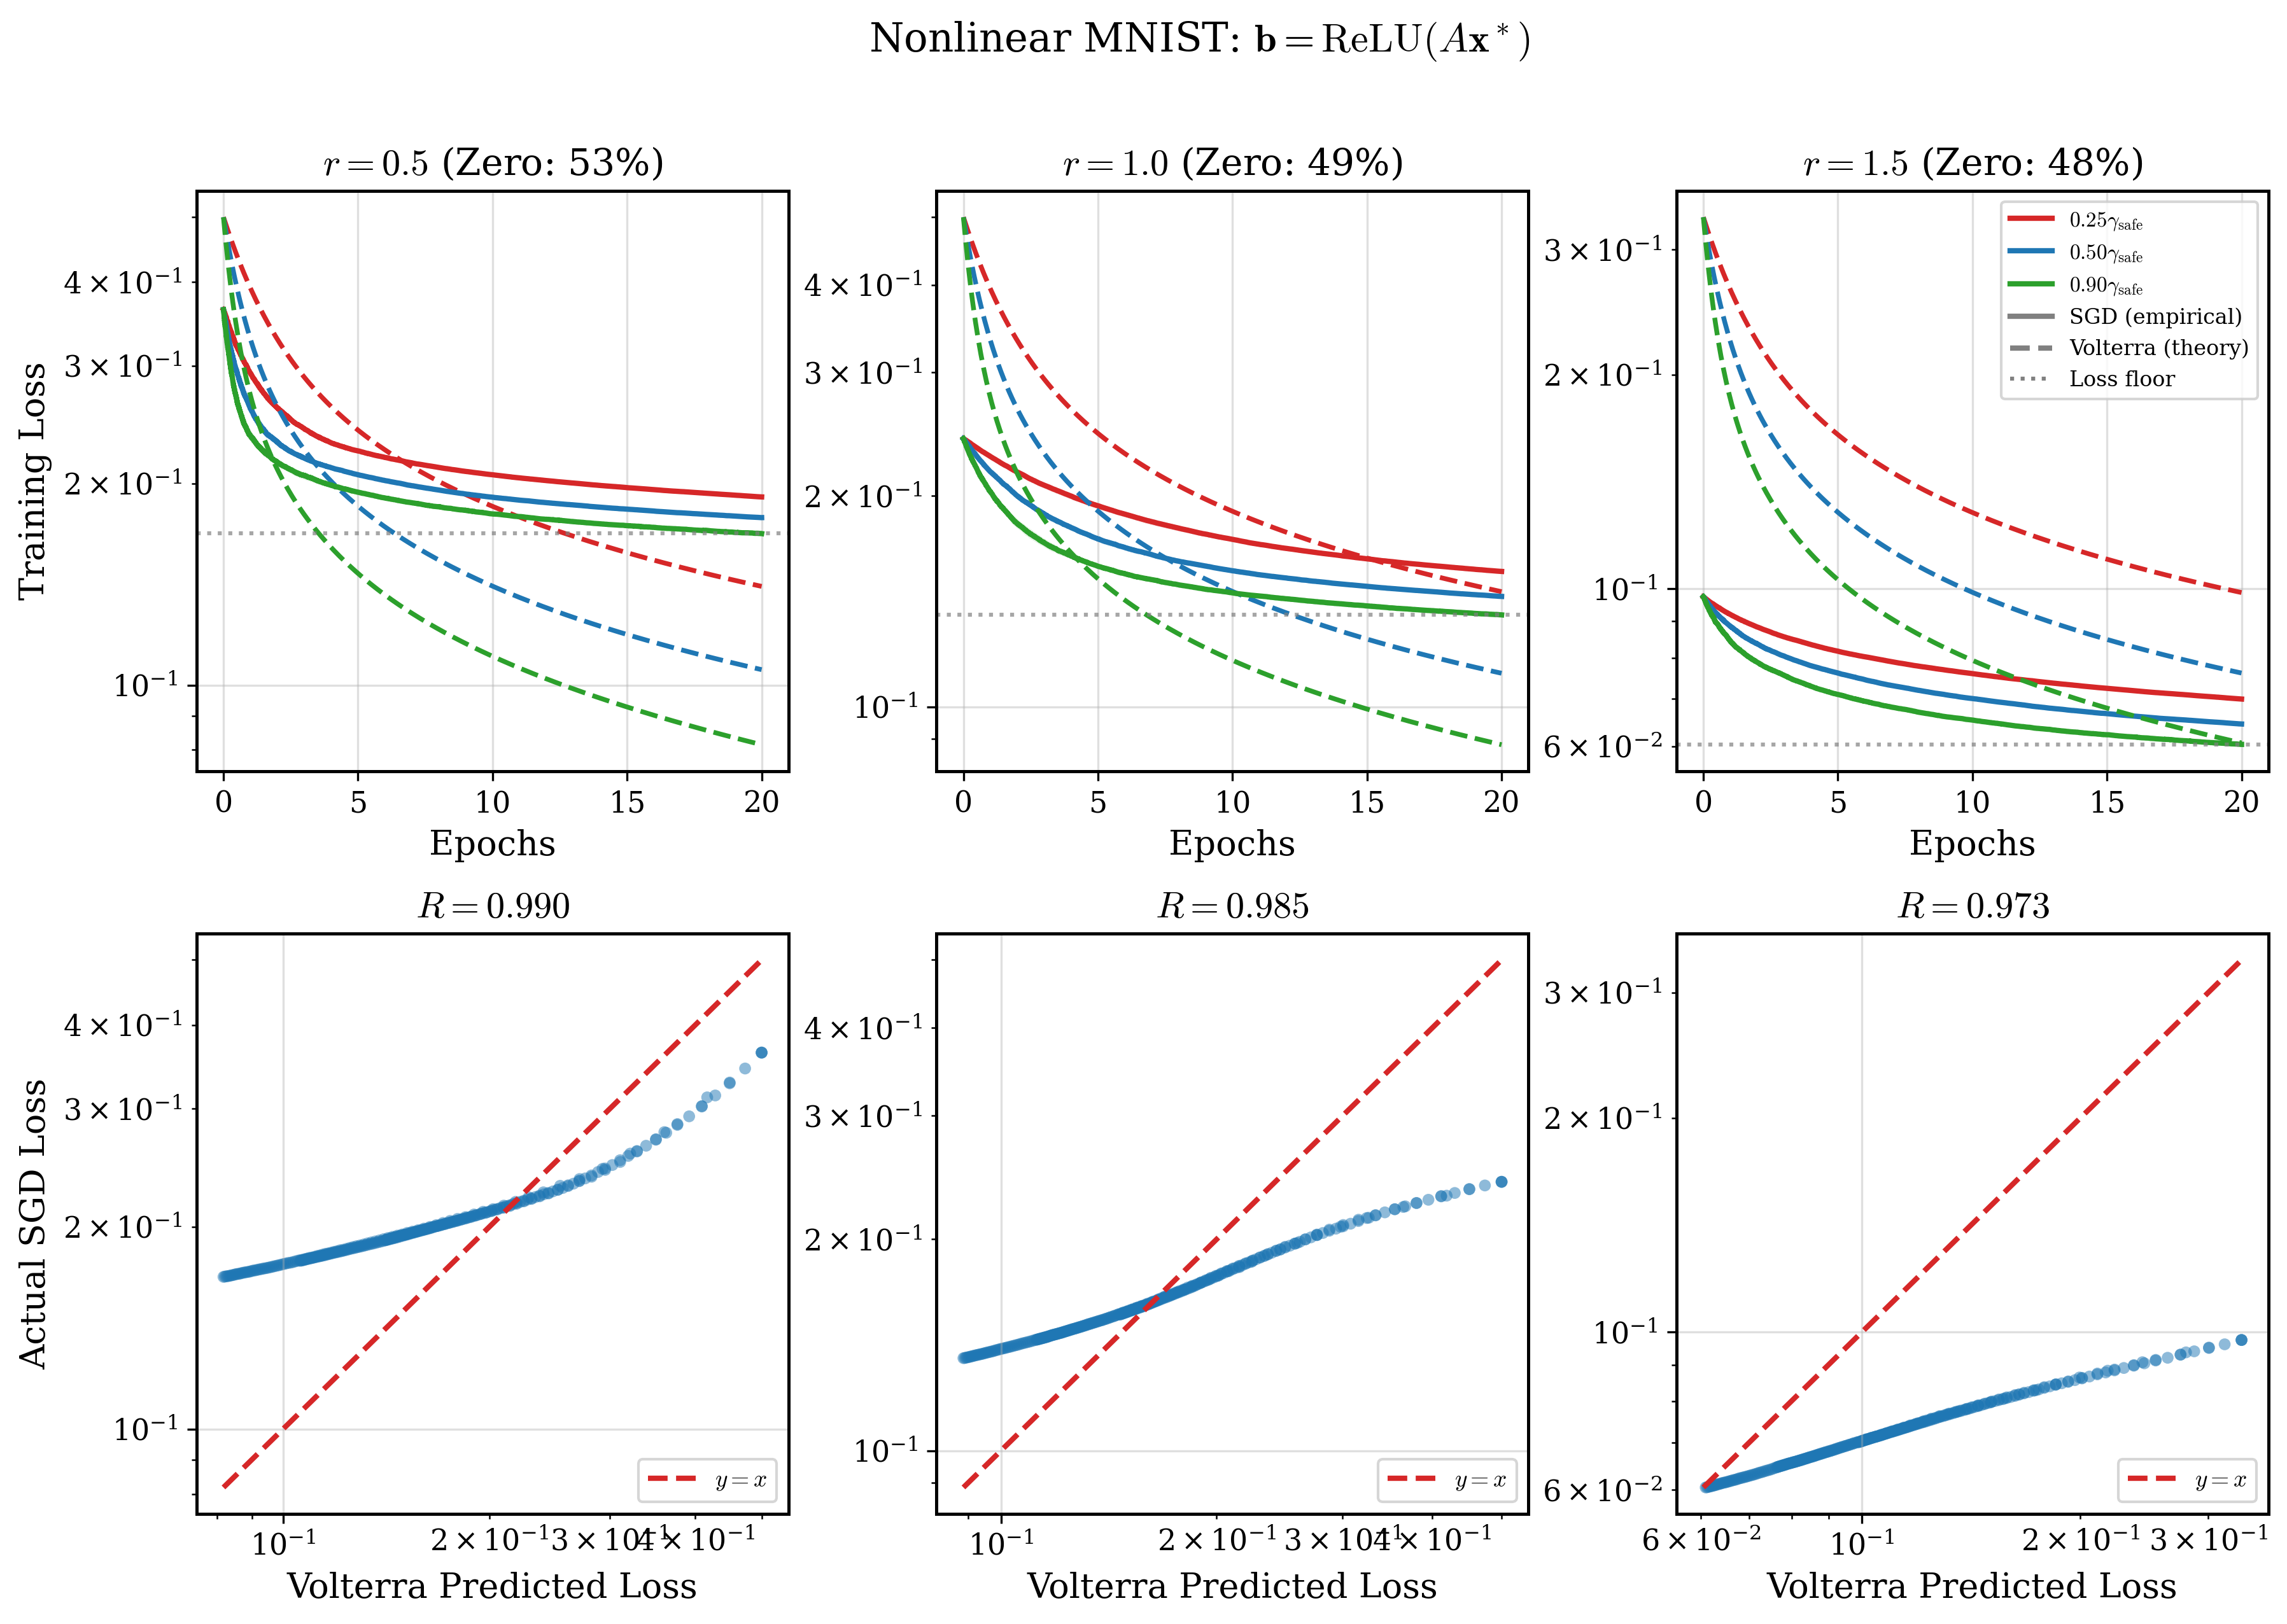
\includegraphics[width=0.95\linewidth]{fig3_nonlinear_mnist.png}
\end{center}
\vspace{-0.2cm}
\small \textit{$\sim$50\% of targets clipped to zero. Loss floor emerges. Still $R > 0.97$.}

\end{block}

% --- 6. WHITENING & CRITICALITY ---
\begin{block}{6. Whitening \& Step-Size Criticality}
\justifying

\textbf{(c) Whitened MNIST:} $\tilde{A} = A\Sigma^{-1/2}$ reduces spectral ratio
\vspace{0.1cm}
\begin{center}
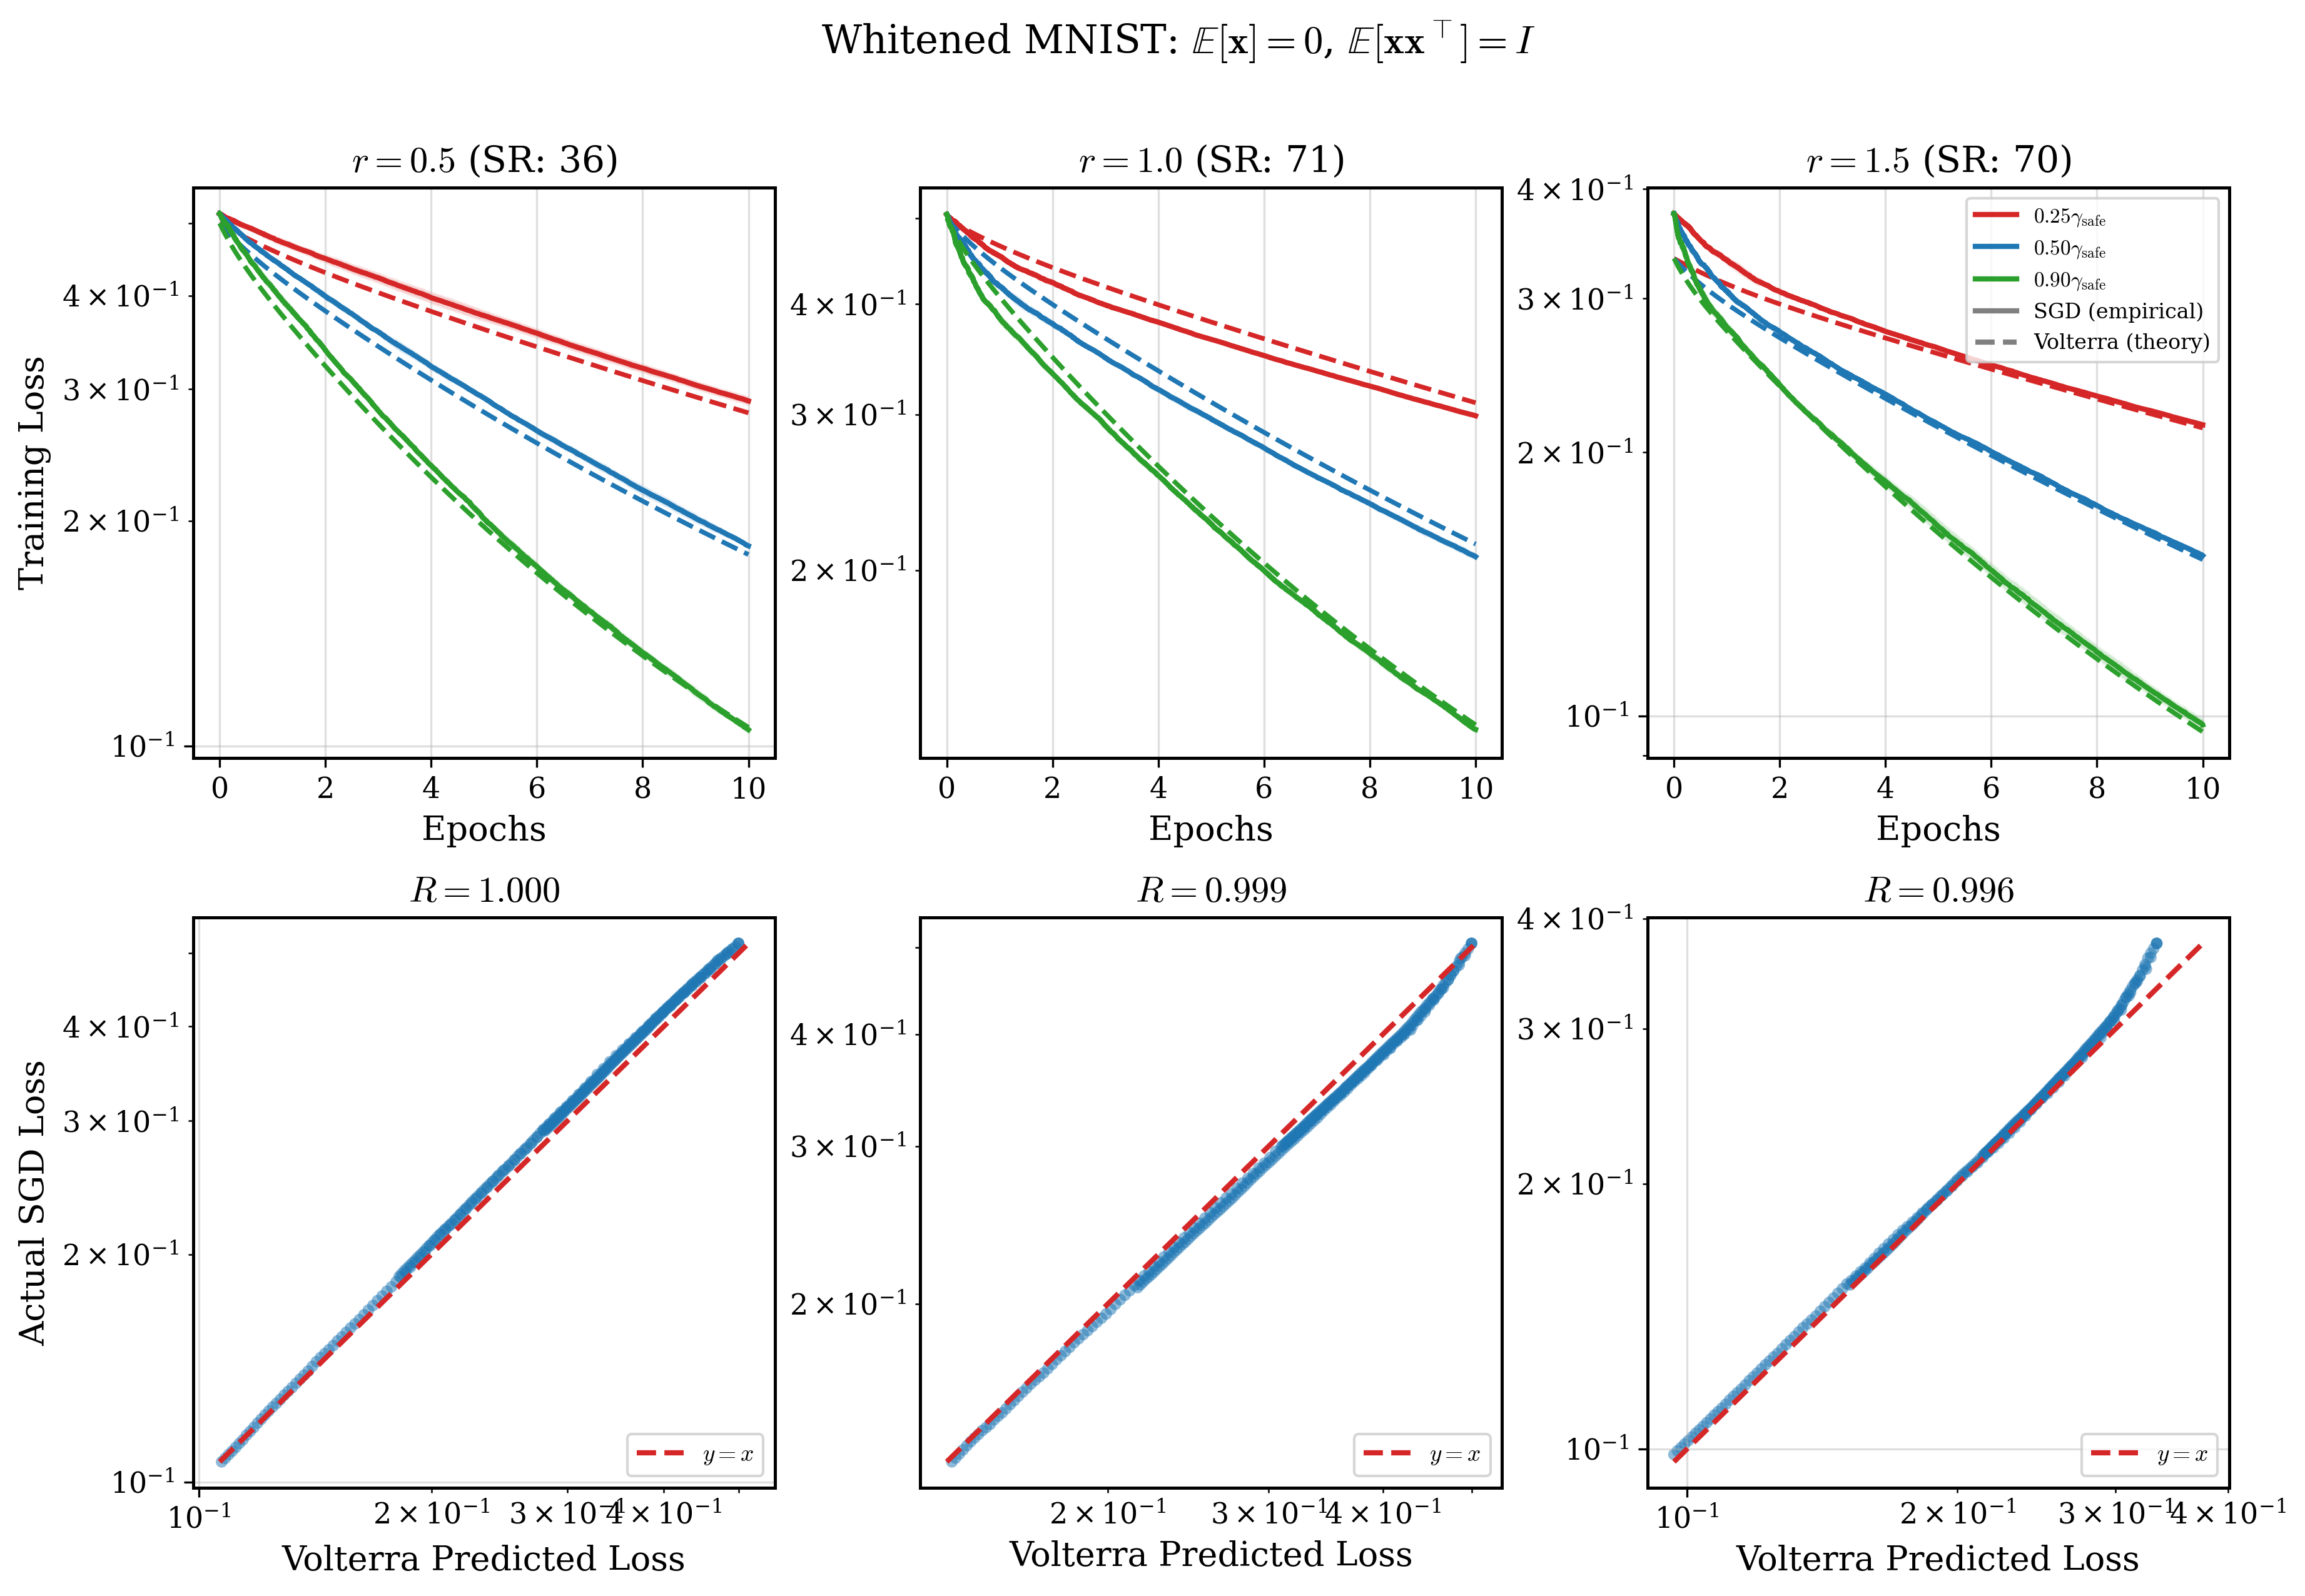
\includegraphics[width=0.95\linewidth]{fig4_whitened_mnist.png}
\end{center}
\vspace{-0.2cm}
\small \textit{Whitening: SR drops from $\sim$270 to $\sim$36-71. Near-perfect $R \approx 0.999$.}

\vspace{0.3cm}
\textbf{(d) Step-Size Criticality Analysis:}
\vspace{0.1cm}
\begin{center}
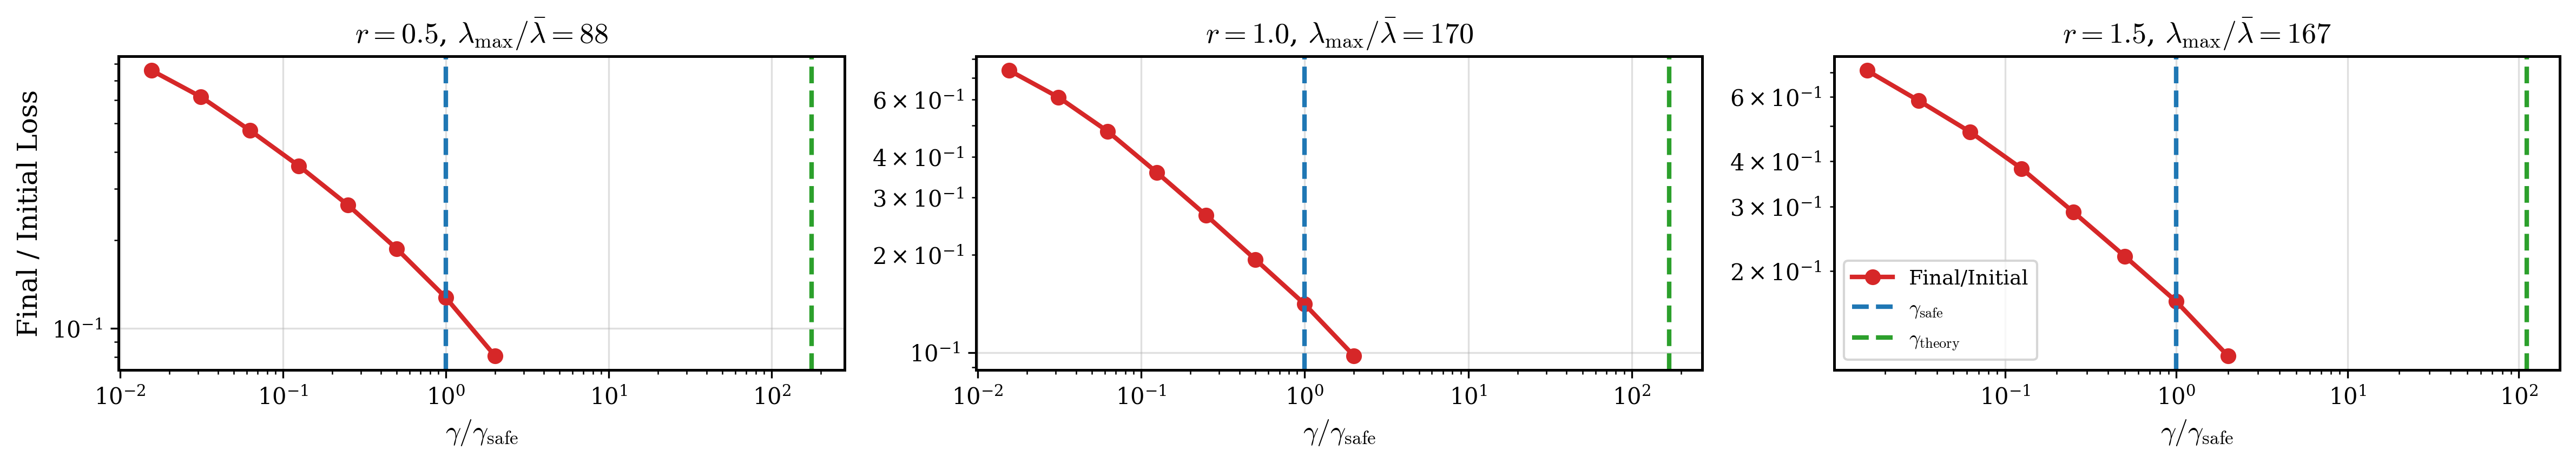
\includegraphics[width=0.95\linewidth]{fig5_criticality.png}
\end{center}
\vspace{-0.2cm}
\small \textit{Large spectral ratio ($\lambda_{\max}/\bar{\lambda} \sim 170$) causes $\gamma_{\text{theory}}$ to overestimate safe step size.}

\end{block}

\end{column}
\end{columns}

\end{frame}
\end{document}
